\documentclass[10pt]{article}
\usepackage{pgfplots, times}
\usepackage{amsmath, amsfonts, amssymb, bm, color, graphicx}
\usepackage{algorithm2e, nicefrac, siunitx}
\usepackage[paperwidth=14cm,paperheight=10cm,lmargin=0in,rmargin=0in,tmargin=0.in,bmargin=0.in]{geometry}
\usetikzlibrary{positioning, shapes, calc} 	

\newlength\figwidth
\newlength\figheight
\newlength\hfigsep
\newlength\vfigsep

\setlength{\figwidth}{7.0cm}
\setlength{\hfigsep}{5ex}
\setlength{\vfigsep}{1em}

\pgfplotsset{
  compat=newest,
  plotStyle/.style= {
    xmin = 21.85,
    xmax = 23.85,
    ymin = 4.3,
    ymax = 5.3,
    minor tick num=1,
    width=\figwidth,
    axis on top,
    xlabel = {$x\, (\si{mm})$},
    ylabel = {$y\, (\si{mm})$},
    y label style={fill=white},    
    xtick pos=left,
    ytick pos=left,
    tick align = outside,
    tick style={black},
    axis line style={black},
  },
  noYticks/.style = {
    yticklabels={},
    ylabel = {},
  },
  noXticks/.style = {
    xticklabels={},
    xlabel = {},
  },
  topXticks/.style = {
    xtick pos=right,
    xticklabel pos=right,
  }  
}

\begin{document}
\flushleft
\begin{tikzpicture}[font=\footnotesize]
  \begin{axis}[
      alias=full,
      plotStyle,
      width=2\figwidth,
      xmin = 0.0,
      xmax = 40.0,
      ymin = 0.0,
      ymax = 10.0,
      topXticks,
      anchor=north west,
      axis equal image]
    \addplot graphics[xmin=0.0, xmax=40.0,ymin=0.0, ymax=10.0] {./sim_raw/square_30kv/field_9500_1909_full};
    \draw[thick, fill=black, fill opacity=0.0](axis cs: 21.85,4.2) rectangle ++(2,1);
    \node[fill=white, thick, draw=black, anchor=north east]  at (rel axis cs: 0.95, 0.95) {$t = 19.1\,\si{ns}$};

    \node[alias=c1,inner sep=0pt] at (axis cs:21.85,5.2) {};
    \node[alias=c2,inner sep=0pt] at (axis cs:23.85,4.2) {};        
  \end{axis}
  
  \begin{axis}[
      alias=field1,
      at=(full.south west),
      yshift=-5em,
      plotStyle,
      anchor=north west,
      axis equal image]
    \addplot graphics[xmin=21.85, xmax=23.85,ymin=4.3, ymax=5.3] {./sim_raw/square_30kv/field_9500_1909_view3};
%    \node[fill=white, draw=black, anchor=north west]  at (rel axis cs: 0.05, 0.95) {a)};
%    \node[fill=white, thick, draw=black, anchor=north east]  at (rel axis cs: 0.95, 0.95) {$t = 19.1\,\si{ns}$};                        
  \end{axis}

  \draw[densely dashed, black, thick] (c1) -- (field1.north west);
  \draw[densely dashed, black, thick] (c2) -- (field1.south east);    

  \begin{axis}[
      alias=electrons1,
      at=(full.south east),
      yshift=-5em,      
      anchor=north east,
      plotStyle,
      axis equal image]
    \addplot graphics[xmin=21.85, xmax=23.85,ymin=4.3, ymax=5.3] {./sim_raw/square_30kv/electrons_9500_1909_view3};
%    \node[fill=white, draw=black, anchor=north west]  at (rel axis cs: 0.05, 0.95) {f)};                    
  \end{axis}
  
  %% Colorbar for field
  \node[alias=colorbar, anchor=south west, inner sep=0pt,yshift=1em] at ($(field1.north west)!0.0!(field1.north east)$) {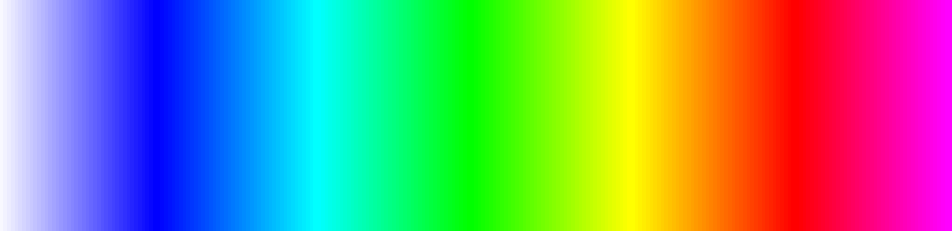
\includegraphics[width=4cm, height=5mm]{./sim_raw/colorbar_calewhite}};
  \draw[thick] ([xshift= 0.1ex]colorbar.north west) -- ++ (0,1.5ex) node[anchor=south,] {$0.0$};
  \draw[thick] ([xshift= -0.1ex]colorbar.north east) -- ++ (0,1.5ex) node[anchor=south,] {$4.5$};
  \draw[thick] ($(colorbar.north west)!0.25!(colorbar.north east)$) -- ++ (0,1.5ex) node[anchor=south,] {$1.125$};
  \draw[thick] ($(colorbar.north west)!0.5!(colorbar.north east)$) -- ++ (0,1.5ex) node[anchor=south,fill=white] {$2.25$};
  \draw[thick] ($(colorbar.north west)!0.75!(colorbar.north east)$) -- ++ (0,1.5ex) node[anchor=south,fill=white] {$3.375$};
  \node[anchor=north west, inner sep=2pt] at ([yshift=1ex]colorbar.north east) {$\times 10^{7}\,\textrm{V/m}$};

  %% Colorbar for electrons
  \node[alias=colorbar, anchor=south west, inner sep=0pt,yshift=1em] at ($(electrons1.north west)!0.0!(electrons1.north east)$) {
\includegraphics[width=4cm, height=5mm]{./sim_raw/colorbar_plasma}};
  \draw[thick] ([xshift= 0.1ex]colorbar.north west) -- ++ (0,1.5ex) node[anchor=south,fill=white] {$0.0$};
  \draw[thick] ([xshift= -0.1ex]colorbar.north east) -- ++ (0,1.5ex) node[anchor=south,] {$1.0$};
  \draw[thick] ($(colorbar.north west)!0.25!(colorbar.north east)$) -- ++ (0,1.5ex) node[anchor=south,] {$0.25$};
  \draw[thick] ($(colorbar.north west)!0.5!(colorbar.north east)$) -- ++ (0,1.5ex) node[anchor=south,] {$0.5$};
  \draw[thick] ($(colorbar.north west)!0.75!(colorbar.north east)$) -- ++ (0,1.5ex) node[anchor=south,] {$0.75$};
  \node[anchor=north west, inner sep=2pt] at ([yshift=1ex]colorbar.north east) {$\times 10^{20}\,\si{m}^{-3}$};
\end{tikzpicture}



\end{document}
